\documentclass[11pt]{article}

\usepackage[T1]{fontenc}
\usepackage[utf8]{inputenc}
\usepackage{mathpazo}
\usepackage{amsmath,amssymb,amsthm,mathtools}
\usepackage[margin=1.05in]{geometry}
\usepackage{microtype}
\usepackage{enumitem}
\usepackage{booktabs}
\usepackage{xcolor}
\usepackage{titlesec}
\usepackage{fancyhdr}
\usepackage{tikz}
\usepackage{pgfplots}
\pgfplotsset{compat=1.17}
\usetikzlibrary{arrows.meta,positioning,calc,decorations.pathmorphing,backgrounds}
\usepackage{tcolorbox}
\tcbuselibrary{skins,breakable}
\usepackage[colorlinks=true,allcolors=accent]{hyperref}
\usepackage{url}
\urlstyle{same}

% ---------------------------------------------------------------- colours
\definecolor{accent}{HTML}{1D4E89}
\definecolor{accentlight}{HTML}{EAF0F7}
\definecolor{rule}{HTML}{C8D2DE}
\definecolor{warm}{HTML}{A8442A}
\definecolor{warmlight}{HTML}{FBF0EC}

% ---------------------------------------------------------------- headings
\titleformat{\section}{\large\bfseries\color{accent}}{\thesection.}{0.6em}{}
\titlespacing*{\section}{0pt}{1.6\baselineskip}{0.5\baselineskip}
\titleformat{\subsection}{\normalsize\bfseries}{\thesubsection}{0.6em}{}
\titlespacing*{\subsection}{0pt}{1.1\baselineskip}{0.35\baselineskip}

\pagestyle{fancy}
\fancyhf{}
\renewcommand{\headrulewidth}{0.4pt}
\renewcommand{\headrule}{\hbox to\headwidth{\color{rule}\leaders\hrule height \headrulewidth\hfill}}
\lhead{\footnotesize\color{accent}PHYS-GA 2043 \;\textbullet\; Machine Learning for Scientists}
\rhead{\footnotesize\color{accent}Lecture 1}
\cfoot{\footnotesize\thepage}

% ---------------------------------------------------------------- boxes
\newtcolorbox{keybox}[1][]{
  enhanced, breakable, colback=accentlight, colframe=accent,
  boxrule=0pt, leftrule=2.5pt, arc=1pt, left=10pt, right=10pt, top=7pt, bottom=7pt,
  fonttitle=\bfseries\color{accent}, coltitle=accent,
  attach boxed title to top left={yshift=-2mm,xshift=8pt},
  boxed title style={colback=accentlight,boxrule=0pt,arc=0pt},
  #1}

\newtcolorbox{asidebox}[1][]{
  enhanced, breakable, colback=warmlight, colframe=warm,
  boxrule=0pt, leftrule=2.5pt, arc=1pt, left=10pt, right=10pt, top=7pt, bottom=7pt,
  #1}

\newtcolorbox{algbox}[1]{
  enhanced, breakable, colback=white, colframe=rule, boxrule=0.6pt, arc=2pt,
  left=10pt, right=10pt, top=8pt, bottom=8pt,
  title={\color{accent}\bfseries #1}, fonttitle=\bfseries,
  colbacktitle=accentlight, coltitle=accent, titlerule=0pt,
  attach boxed title to top left={yshift=-2.6mm,xshift=10pt},
  boxed title style={boxrule=0pt,arc=1pt}}

% ---------------------------------------------------------------- macros
\DeclareMathOperator*{\argmin}{arg\,min}
\newcommand{\R}{\mathbb{R}}
\newcommand{\Loss}{\mathcal{L}}
\newcommand{\yhat}{\hat{y}}
\newcommand{\bs}[1]{\boldsymbol{#1}}
\newcommand{\board}[1]{\footnote{\textit{Board note:} #1}}

\setlist[itemize]{itemsep=2pt,topsep=4pt,leftmargin=1.4em}
\setlist[enumerate]{itemsep=2pt,topsep=4pt,leftmargin=1.7em}

\begin{document}

% ================================================================ TITLE
\begin{center}
{\color{accent}\rule{\textwidth}{1.2pt}}\\[9pt]
{\normalsize\color{accent}\scshape Lecture 1 \;\textbullet\; Tuesday 8 September 2026}\\[8pt]
{\LARGE\bfseries Multilayer Perceptrons and Optimisation}\\[7pt]
{\large\itshape neural networks, and the problem of finding them}\\[9pt]
{\normalsize Carolina Cuesta-Lazaro \;\textbullet\; PHYS-GA 2043}\\[6pt]
{\footnotesize\color{black!60} Transcribed and typeset by Claude from the lecture board notes}\\[8pt]
{\color{accent}\rule{\textwidth}{0.5pt}}
\end{center}

\vspace{0.2em}

% ================================================================ 0
\section{This week in AI4Science}

\begin{tcolorbox}[enhanced, colback=white, colframe=rule, boxrule=0.6pt, arc=2pt,
  left=10pt, right=10pt, top=7pt, bottom=7pt]
\small
\textbf{Links shown in class}
\begin{itemize}[leftmargin=1.2em, itemsep=1pt]
  \item T. Buckmaster, statement of 8 September 2026 (Courant Institute) ---
        \url{https://cims.nyu.edu/~tristanb/statement.pdf}
  \item OpenAI, \emph{On the Navier--Stokes Millennium Prize Problem} ---
        \url{https://openai.com/index/navier-stokes-solution/}
  \item \emph{Quanta Magazine}, 8 September 2026 ---
        \url{https://www.quantamagazine.org/ai-has-solved-one-of-maths-1-million-millennium-prize-problems-20260908/}
\end{itemize}
\end{tcolorbox}

\noindent
Both announcements came out on the morning of this lecture.

\medskip
\noindent
Buckmaster (NYU Courant) and Alpöge (Anthropic) published proofs of finite-time blowup
with smooth forcing for incompressible porous media, Boussinesq, and 3D incompressible
Euler. They used AI models throughout and verified the results in Lean. Twelve hours
later OpenAI announced a proof of a finite-time singularity for forced 3D Navier--Stokes,
also formalised in Lean, obtained by about $10^{4}$ agents running for 88 hours, plus 17
hours to formalise. The two groups then disputed priority; the links cover both sides.

\medskip
\noindent
Lean is a proof assistant. It reduces every step of an argument to a small fixed set of
axioms and checks those steps mechanically, so we can know a proof is correct even when it
is far too long for anyone to read.

% ================================================================ 1
\section{The supervised learning problem}

We are given pairs of \textbf{features} and \textbf{labels}.
%
\[
  x \in \R^{m} \quad\text{(features)},
  \qquad\qquad
  y \in \R^{n} \quad\text{(labels)}.
\]
%
We want a function that maps one to the other. We do not know it, so we choose a family
of candidate functions indexed by parameters $\theta$ and search inside that family:
%
\[
  \yhat = f_\theta(x), \qquad f_\theta : \R^m \to \R^n .
\]
%
A \textbf{loss} $\Loss(\theta; y, \yhat)$ measures how good a given $\theta$ is.
Training means minimising it.

\begin{center}
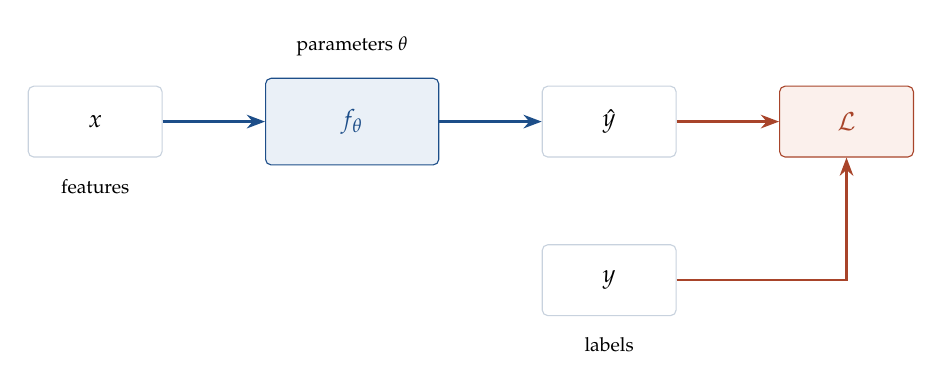
\begin{tikzpicture}[
    node distance=13mm, >=Stealth,
    box/.style={draw=rule, fill=white, rounded corners=2pt, minimum height=9mm,
                minimum width=17mm, font=\small},
    model/.style={draw=accent, fill=accentlight, rounded corners=2pt, minimum height=11mm,
                minimum width=22mm, font=\small\bfseries, text=accent}]
  \node[box] (x) {$x$};
  \node[model, right=of x] (f) {$f_\theta$};
  \node[box, right=of f] (yh) {$\yhat$};
  \node[box, below=11mm of yh] (y) {$y$};
  \node[draw=warm, fill=warmlight, rounded corners=2pt, minimum height=9mm,
        minimum width=17mm, font=\small, text=warm, right=of yh] (l) {$\Loss$};
  \draw[->, thick, accent] (x) -- (f);
  \draw[->, thick, accent] (f) -- (yh);
  \draw[->, thick, warm] (yh) -- (l);
  \draw[->, thick, warm] (y) -| (l);
  \node[font=\scriptsize, below=1.5mm of x] {features};
  \node[font=\scriptsize, below=1.5mm of y] {labels};
  \node[font=\scriptsize, above=1.5mm of f] {parameters $\theta$};
\end{tikzpicture}
\end{center}

\noindent
This leaves two questions. What should $f_\theta$ look like (Sections
\ref{sec:linear}--\ref{sec:mlp}), and how do we search for $\theta$ (Sections
\ref{sec:found}--\ref{sec:muon})?

\begin{center}
\small
\begin{tabular}{@{}ll@{\hspace{2.2em}}ll@{}}
\toprule
$m$ & input dimension & $D$ & number of parameters \\
$n$ & output dimension & $g_t$ & gradient at step $t$ \\
$L$ & number of layers (depth) & $\eta$ & learning rate / step size \\
$\theta$ & all parameters, $\theta \in \R^D$ & $B$ & minibatch size \\
$\Loss$ & loss & $\varepsilon$ & small constant, $\sim 10^{-8}$ \\
\bottomrule
\end{tabular}
\end{center}

% ================================================================ 2
\section{The simplest choice, and why it fails}
\label{sec:linear}

Start with the smallest family that maps $\R^m$ to $\R^n$: an affine
map.\board{On the board $W$ was labelled $m\times n$; here it is written $n \times m$ so
that $Wx$ has the shape of $y$.}
%
\[
  f_\theta(x) = W x + b,
  \qquad W \in \R^{n\times m}, \quad b \in \R^{n},
  \qquad \theta = \{W, b\}.
\]

\noindent
This can be solved in closed form, but it can only represent a linear function. The
obvious way to make it richer is to stack several of them. That does not work. Compose
two layers:
%
\[
  f_2\big(f_1(x)\big) = W_2 (W_1 x + b_1) + b_2
  = \underbrace{(W_2 W_1)}_{\tilde{W}} x + \underbrace{(W_2 b_1 + b_2)}_{\tilde{b}},
\]
%
which is again of the form $\tilde W x + \tilde b$. Induction extends this to any depth:
%
\[
  f_L\Big(f_{L-1}\big(\cdots f_1(x) \cdots \big)\Big)
  \;=\; W_{\mathrm{eff}}\, x + b_{\mathrm{eff}},
  \qquad W_{\mathrm{eff}} = W_L W_{L-1}\cdots W_1,
  \qquad \theta = \{\theta_1,\dots,\theta_L\}.
\]

\begin{keybox}
A composition of affine maps is an affine map. An $L$-layer linear network represents
the same set of functions as a single linear layer, using $L$ times as many parameters.
Depth on its own adds nothing.
\end{keybox}

\noindent
If an intermediate layer is narrow, the rank of $W_{\mathrm{eff}}$ is limited by it, and
the stack represents less than a single layer would. We therefore need something between
the layers to stop them collapsing.

% ================================================================ 3
\section{The perceptron}

We insert a nonlinearity, a scalar function $A$ applied elementwise:
%
\[
  f_\theta(x) = A\big(W x + b\big), \qquad \theta = \{W, b\}.
\]
%
$A$ is the \textbf{activation}. Two common choices:

\subsection*{Sigmoid}

\[
  \sigma(x) = \frac{1}{1 + e^{-x}}
\]

\begin{center}
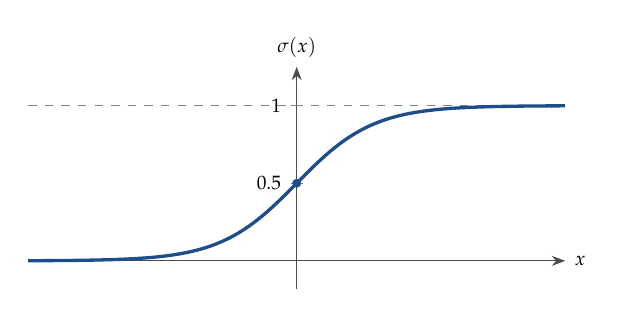
\begin{tikzpicture}
\begin{axis}[
  width=8.4cm, height=4.4cm,
  axis lines=middle, xlabel={$x$}, ylabel={$\sigma(x)$},
  every axis x label/.style={at={(ticklabel* cs:1.0)},anchor=west},
  every axis y label/.style={at={(ticklabel* cs:1.0)},anchor=south},
  xmin=-7, xmax=7, ymin=-0.18, ymax=1.25,
  ytick={0.5,1}, yticklabels={$0.5$,$1$}, xtick={0}, xticklabels={$0$},
  tick label style={font=\scriptsize},
  label style={font=\scriptsize},
  axis line style={-Stealth, draw=black!70}]
  \addplot[dashed, gray, domain=-7:7, samples=2]{1};
  \addplot[accent, very thick, domain=-7:7, samples=120]{1/(1+exp(-x))};
  \addplot[only marks, mark=*, mark size=1.4pt, accent] coordinates {(0,0.5)};
\end{axis}
\end{tikzpicture}
\end{center}

\noindent
The sigmoid is smooth and monotone and maps $\R$ to $(0,1)$, with
$\sigma(0) = \tfrac12$. Its derivative $\sigma' = \sigma(1-\sigma)$ is at most $\tfrac14$
and goes to zero in both tails, so the sigmoid saturates. This matters later: when we
differentiate through $L$ layers next lecture, this factor appears $L$ times.

\subsection*{ReLU}

\[
  \mathrm{ReLU}(x) = \begin{cases} x, & x > 0 \\ 0, & x \le 0 \end{cases}
\]

\begin{center}
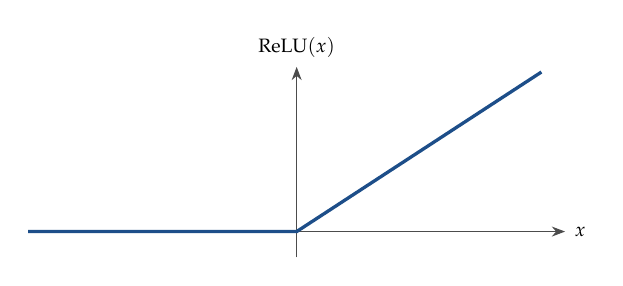
\begin{tikzpicture}
\begin{axis}[
  width=8.4cm, height=4.0cm,
  axis lines=middle, xlabel={$x$}, ylabel={$\mathrm{ReLU}(x)$},
  every axis x label/.style={at={(ticklabel* cs:1.0)},anchor=west},
  every axis y label/.style={at={(ticklabel* cs:1.0)},anchor=south},
  xmin=-3.4, xmax=3.4, ymin=-0.5, ymax=3.2,
  xtick={0}, xticklabels={$0$}, ytick=\empty,
  tick label style={font=\scriptsize}, label style={font=\scriptsize},
  axis line style={-Stealth, draw=black!70}]
  \addplot[accent, very thick] coordinates {(-3.4,0) (0,0) (3.1,3.1)};
\end{axis}
\end{tikzpicture}
\end{center}

\noindent
ReLU is piecewise linear, its derivative is $0$ or $1$, it does not saturate for $x>0$,
and it is cheap to evaluate. It is not differentiable at the origin, which does not cause
problems in practice. Any non-polynomial $A$ prevents the collapse of Section
\ref{sec:linear}.

% ================================================================ 4
\section{The multilayer perceptron}
\label{sec:mlp}

With a nonlinearity in place, stacking layers does add expressive power. Writing
$f_{\theta_\ell}(u) = A_\ell(W_\ell u + b_\ell)$ for one layer:
%
\[
  f_\theta(x) = f_{\theta_L}\Big(f_{\theta_{L-1}}\big(\cdots f_{\theta_1}(x)\cdots\big)\Big),
  \qquad \theta = \{\theta_1, \ldots, \theta_L\}.
\]
%
$L$ is the \textbf{depth} and the number of rows of $W_\ell$ is the \textbf{width} of
layer $\ell$. Layers between the input and the output are called hidden. The last layer
usually has no activation for regression, or a softmax for classification.

\begin{center}
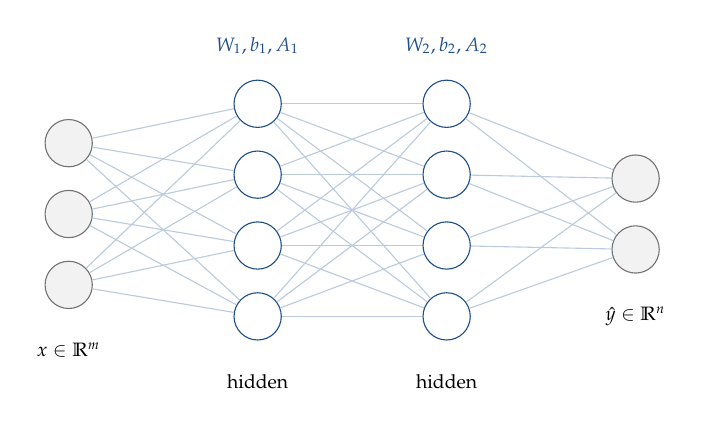
\begin{tikzpicture}[
  >=Stealth,
  nd/.style={circle, draw=accent, fill=white, minimum size=6mm, inner sep=0pt},
  ndi/.style={circle, draw=black!55, fill=black!5, minimum size=6mm, inner sep=0pt}]
  \foreach \i in {1,2,3} \node[ndi] (i\i) at (0, 1.4-0.9*\i) {};
  \foreach \i in {1,2,3,4} \node[nd] (h\i) at (2.4, 1.9-0.9*\i) {};
  \foreach \i in {1,2,3,4} \node[nd] (k\i) at (4.8, 1.9-0.9*\i) {};
  \foreach \i in {1,2} \node[ndi] (o\i) at (7.2, 0.95-0.9*\i) {};
  \foreach \a in {1,2,3} \foreach \b in {1,2,3,4}
     \draw[draw=accent!30] (i\a) -- (h\b);
  \foreach \a in {1,2,3,4} \foreach \b in {1,2,3,4}
     \draw[draw=accent!30] (h\a) -- (k\b);
  \foreach \a in {1,2,3,4} \foreach \b in {1,2}
     \draw[draw=accent!30] (k\a) -- (o\b);
  \node[font=\scriptsize, below=3mm of i3] {$x \in \R^m$};
  \node[font=\scriptsize, below=3mm of h4] {hidden};
  \node[font=\scriptsize, below=3mm of k4] {hidden};
  \node[font=\scriptsize, below=3mm of o2] {$\yhat \in \R^n$};
  \node[font=\scriptsize, accent, above=2mm of h1] {$W_1, b_1, A_1$};
  \node[font=\scriptsize, accent, above=2mm of k1] {$W_2, b_2, A_2$};
\end{tikzpicture}
\end{center}

% ================================================================ 5
\section{The universal approximation theorem}

Is this family rich enough? Yes.

\begin{keybox}[title={Universal approximation}]
A feedforward network with a \emph{single hidden layer} and a suitable non-polynomial
activation can approximate any continuous function on a compact subset of $\R^m$ to any
desired accuracy, given enough hidden units.
\end{keybox}

\noindent
It is easy to read more into this than it says. The question put to the class was:

\begin{center}
{\large\itshape What doesn't it say?}
\end{center}

\begin{asidebox}
\begin{enumerate}[label=\textbf{\arabic*.}]
  \item \textbf{It does not say the solution can be found.} The theorem says a good
  $\theta$ exists somewhere in $\R^D$. Whether a procedure starting from a random
  initialisation reaches it is a separate question.
  \item \textbf{It does not say the solution will generalise.} The approximation is
  guaranteed on the region where we match the function, and says nothing about points
  outside it.
\end{enumerate}
It also says nothing about cost, since ``enough hidden units'' can mean exponentially
many, and it gives no reason to prefer depth, which is what works in practice. What makes
the problem tractable is choosing an architecture whose structure matches the structure of
the data. These are the inductive biases, and we take them up from Lecture 3 onwards.
\end{asidebox}

\noindent
Those two gaps are the syllabus:

\begin{center}
\small
\begin{tabular}{@{}lll@{}}
\toprule
\textbf{Gap} & \textbf{Question} & \textbf{Where} \\
\midrule
Can it be found? & optimisation --- find a good $\theta$ as fast as possible & rest of this lecture \\
Will it generalise? & regularisation, capacity, double descent & Lecture 2 onwards \\
\bottomrule
\end{tabular}
\end{center}

\noindent
Today we deal with the first one.

% ================================================================ 6
\section{Can it be found?}
\label{sec:found}

Formally, we want
%
\[
  \theta^{\star} \in \argmin_{\theta \in \Theta \subseteq \R^{D}} \Loss(\theta),
\]
%
where $D$, the number of parameters, is typically in the millions or billions. The loss
surface is not convex:

\begin{center}
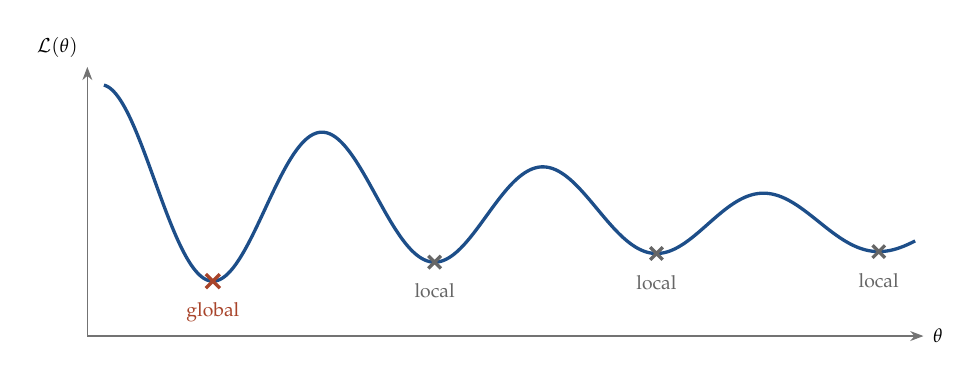
\begin{tikzpicture}
\begin{axis}[
  width=12.2cm, height=5.0cm,
  axis lines=left, xtick=\empty, ytick=\empty,
  xlabel={$\theta$}, ylabel={$\Loss(\theta)$},
  every axis x label/.style={at={(ticklabel* cs:1.0)},anchor=west,font=\scriptsize},
  every axis y label/.style={at={(ticklabel* cs:1.0)},anchor=south east,font=\scriptsize},
  axis line style={-Stealth, draw=black!55},
  xmin=-0.2, xmax=9.9, ymin=-1.75, ymax=1.95,
  clip=false]
  \addplot[accent, very thick, domain=0:9.8, samples=400]
    {1.45*cos(deg(2.35*x))*exp(-0.16*x) - 0.055*x + 0.25};
  % global minimum
  \addplot[only marks, mark=x, mark size=3.6pt, very thick, warm]
    coordinates {(1.316,-0.996)};
  \node[font=\scriptsize, warm, below=1.5mm] at (axis cs:1.316,-0.996) {global};
  % local minima
  \addplot[only marks, mark=x, mark size=3.2pt, very thick, black!60]
    coordinates {(3.995,-0.734) (6.675,-0.615) (9.360,-0.589)};
  \node[font=\scriptsize, black!60, below=1.5mm] at (axis cs:3.995,-0.734) {local};
  \node[font=\scriptsize, black!60, below=1.5mm] at (axis cs:6.675,-0.615) {local};
  \node[font=\scriptsize, black!60, below=1.5mm] at (axis cs:9.360,-0.589) {local};
\end{axis}
\end{tikzpicture}
\end{center}

\noindent
If $\theta^\star$ is a local minimum, then
%
\[
  \nabla \Loss(\theta^{\star}) = 0,
  \qquad\text{and}\qquad
  \nabla^{2} \Loss(\theta^{\star}) \succeq 0,
  \qquad
  H_{ij} = \frac{\partial^{2}\Loss}{\partial \theta_i \, \partial \theta_j},
\]
%
with $H$ positive semi-definite at that point. Both conditions are correct, but neither
helps us here:

\begin{itemize}
  \item $\nabla\Loss(\theta) = 0$ is a system of $D$ coupled nonlinear equations with no
  closed-form solution.
  \item $H$ has $D^{2}$ entries. At $D = 10^{9}$ that is $10^{18}$ numbers, so we cannot
  form it, store it or invert it. Second-order methods are not available at this scale.
\end{itemize}

\noindent
Instead of solving for $\theta^\star$, we iterate, using only first-order information:

\begin{keybox}
\[
  \theta_{t+1} = \theta_{t} + \eta\, d_{t}
\]
\vspace{-1.2em}
\begin{center}
\small $d_t$: descent direction \qquad $\eta$: learning rate, or step size
\end{center}
\end{keybox}

\noindent
Each algorithm below is a different choice of $d_t$ and of how to scale it.

% ================================================================ 7
\section{A wish list}

Before looking at specific algorithms, here is what we want from one.

\begin{center}
\small
\begin{tabular}{@{}p{0.45\textwidth} p{0.45\textwidth}@{}}
\toprule
\textbf{Must have} & \textbf{Nice to have} \\
\midrule
\textbf{1. Converges fast.} Few steps, and each step cheap. Both matter: halving the
number of steps is no good if each one costs ten times as much.
&
\textbf{1. Theoretical guarantees.} Ideally a proof of convergence to a local minimum,
with a rate.
\\[6pt]
\textbf{2. Lightweight in memory.} The state it carries should be a small constant
number of copies of $\theta$. Anything that scales like $D^2$ is unusable.
&
\textbf{2. Robust to the starting point.} Performance should not depend strongly on the
initialisation.
\\[6pt]
&
\textbf{3. Insensitive to hyperparameters.} It should work at its default settings on a
problem nobody has tuned it for.
\\
\bottomrule
\end{tabular}
\end{center}

\begin{asidebox}
The last item may look like a convenience, but it is most of the reason Adam became the
default optimiser. It is rarely the best choice for a given problem, and rarely a bad one
for an unfamiliar problem.
\end{asidebox}

% ================================================================ A1
\section{A1 --- Gradient descent}

\begin{algbox}{A1 \; Gradient descent}
\[
  d_{t} = -\,\nabla_{\theta}\Loss(\theta)\Big|_{\theta_{t}}
  \qquad\Longrightarrow\qquad
  \Loss(\theta + \eta\, d_{t}) < \Loss(\theta)
\]
for $\eta$ small enough.
\end{algbox}

\noindent
A first-order Taylor expansion gives
$\Loss(\theta + \eta d) \approx \Loss(\theta) + \eta\, \nabla\Loss \cdot d$. Choosing
$d = -\nabla\Loss$ makes the correction $-\eta\|\nabla\Loss\|^{2} < 0$, so the loss
decreases as long as $\eta$ is small enough for the expansion to hold. Of all directions
of a fixed length, this one decreases the loss fastest locally. The word ``locally'' is
where the difficulty comes from.

\subsection*{What goes wrong: conditioning}

Take a quadratic with two different curvatures,
%
\[
  f(\theta) = \tfrac{1}{2}\big(\theta_{1}^{2} + \kappa\,\theta_{2}^{2}\big),
  \qquad \kappa > 1 .
\]
%
From a point $\theta$, the direction pointing straight at the minimum is
$-(\theta_{1}, \theta_{2})$. Gradient descent instead moves along
%
\[
  -\nabla f = -(\theta_{1},\, \kappa\,\theta_{2}).
\]
%
The two agree only when $\kappa = 1$. When $\kappa \gg 1$ the steep direction dominates
the gradient, which then points across the valley instead of along it:

\begin{center}
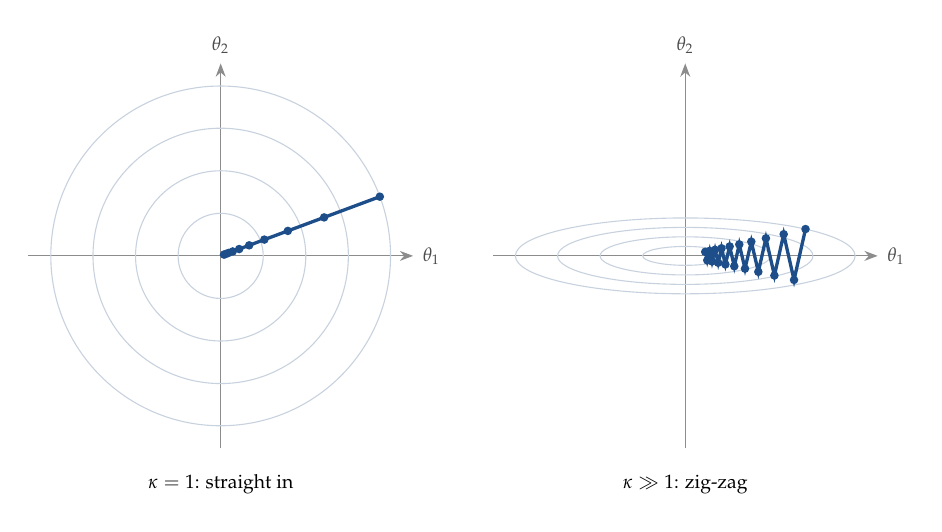
\begin{tikzpicture}[>=Stealth]

% ---------- isotropic panel, equal aspect
\begin{scope}[x=0.235cm, y=0.235cm]
  \draw[black!45,->] (-10.4,0) -- (10.4,0) node[right, font=\scriptsize, black!70] {$\theta_1$};
  \draw[black!45,->] (0,-10.4) -- (0,10.4) node[above, font=\scriptsize, black!70] {$\theta_2$};
  \foreach \r in {2.3,4.6,6.9,9.18}{ \draw[rule] (0,0) circle (\r); }
  \draw[accent, very thick] plot[mark=*, mark size=0.9pt]
    coordinates {(8.60,3.20) (5.59,2.08) (3.63,1.35) (2.36,0.88) (1.54,0.57)
                 (1.00,0.37) (0.65,0.24) (0.42,0.16) (0.27,0.10) (0.18,0.07)};
  \node[font=\scriptsize, below] at (0,-11.3) {$\kappa = 1$: straight in};
\end{scope}

% ---------- anisotropic panel, same aspect
\begin{scope}[xshift=5.9cm, x=0.235cm, y=0.235cm]
  \draw[black!45,->] (-10.4,0) -- (10.4,0) node[right, font=\scriptsize, black!70] {$\theta_1$};
  \draw[black!45,->] (0,-10.4) -- (0,10.4) node[above, font=\scriptsize, black!70] {$\theta_2$};
  \foreach \a/\b in {2.3/0.51, 4.6/1.03, 6.9/1.54, 9.18/2.05}{
    \draw[rule] (0,0) ellipse [x radius=\a, y radius=\b]; }
  \draw[accent, very thick] plot[mark=*, mark size=0.9pt]
    coordinates {(6.50,1.45) (5.88,-1.30) (5.32,1.17) (4.82,-1.06) (4.36,0.95)
                 (3.95,-0.86) (3.57,0.77) (3.23,-0.69) (2.92,0.62) (2.65,-0.56)
                 (2.40,0.51) (2.17,-0.46) (1.96,0.41) (1.78,-0.37) (1.61,0.33)
                 (1.45,-0.30) (1.32,0.27) (1.19,-0.24) (1.08,0.22)};
  \node[font=\scriptsize, below] at (0,-11.3) {$\kappa \gg 1$: zig-zag};
\end{scope}

\end{tikzpicture}
\end{center}

\noindent
The two directions place opposite demands on the step size. Stability along the steep
direction requires $\eta < 2/\kappa$, while progress along the shallow direction goes like
$(1-\eta)^{t}$ and so wants $\eta$ as large as possible. The steep direction therefore
sets the step size and the shallow direction sets the number of steps, and that number
grows with the \textbf{condition number} $\kappa = \lambda_{\max}/\lambda_{\min}$ of the
Hessian. For real loss surfaces $\kappa$ can be in the thousands.

\medskip
\noindent
There is a second problem. $\nabla\Loss$ is a sum over the whole training set, so every
step requires a full pass over the data. Gradient descent fails both of our must-haves.

% ================================================================ A2
\section{A2 --- Momentum}

\begin{algbox}{A2 \; Momentum}
Exponential moving average (EMA) of the gradient $g_t = \nabla_\theta \Loss(\theta_t)$:
\[
  m_{t} = \beta\, m_{t-1} + (1-\beta)\, g_{t},
  \qquad
  \theta_{t} = \theta_{t-1} - \eta\, m_{t}.
\]
\end{algbox}

\noindent
The moving average covers roughly the last $1/(1-\beta)$ gradients, about ten steps at
the usual $\beta = 0.9$. Consider the zig-zag again. The component across the valley
changes sign at every step, so it cancels in the average, while the component along the
valley keeps the same sign and adds up. Momentum therefore damps the oscillation caused by
poor conditioning and speeds up progress along the valley, at the cost of storing one
extra copy of $\theta$.

% ================================================================ A3
\section{A3 --- Stochastic gradient descent}

We can also attack the cost directly, by not computing the exact gradient at all.
Instead we estimate it on a random minibatch of $B$ examples.

\begin{algbox}{A3 \; Stochastic gradient descent}
\[
  \text{error on the gradient} \;\propto\; \frac{1}{\sqrt{B}},
  \qquad\qquad
  \text{cost per step} \;\propto\; B .
\]
\end{algbox}

\noindent
These two scalings are what makes the method work. Halving the error in the gradient
costs four times as much compute, so an accurate gradient is expensive. It also turns out
to be unnecessary: for a fixed compute budget, many cheap noisy steps make more progress
than one exact step. All large models are trained this way.

\subsection*{Where the anisotropy comes from}

Poor conditioning can also come from the data rather than from the loss. Take a linear
model in two features with a squared error:
%
\[
  \yhat = \theta_{1} x_{1} + \theta_{2} x_{2},
  \qquad
  \Loss = \tfrac{1}{2}\,(\yhat - y)^{2},
  \qquad
  e \equiv \yhat - y,
\]
\[
  \frac{\partial \Loss}{\partial \theta_{1}} = e \cdot x_{1},
  \qquad\qquad
  \frac{\partial \Loss}{\partial \theta_{2}} = e \cdot x_{2}.
\]

\noindent
The gradient component for $\theta_{i}$ is proportional to the feature $x_{i}$. So if the
features are physical quantities of very different size, as in the example on the board
with $q$ of order unity, a mass $M \sim 10^{12}$ and a power spectrum
$\mathrm{PS} \sim 10^{4}$, the gradient components differ by twelve orders of magnitude. A
single $\eta$ cannot work for all of them: it either diverges along the large component or
makes no progress along the small one.

\begin{keybox}
The ravine of Section A1 is not a special case. It appears whenever the inputs or the
parameters live at different scales, which for physical data is almost always. There are
two remedies: standardise the features, which you should do in any case, or give the
optimiser a per-dimension step size, which is what A4--A6 do.
\end{keybox}

\subsection*{An aside on the noise: sharp and flat minima}

The noise in the gradient is not only a cost. Consider two minima of the same depth but
different width:

\begin{center}
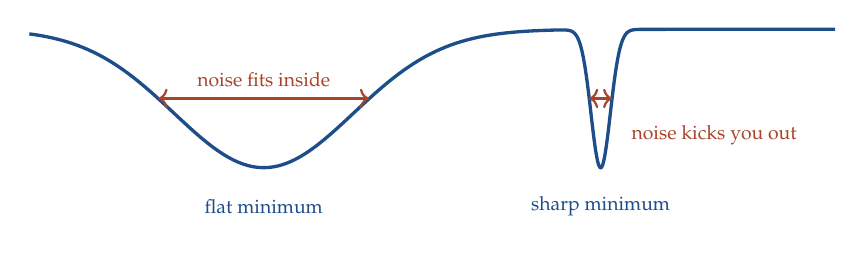
\begin{tikzpicture}
\begin{axis}[
  width=12.0cm, height=4.6cm, axis lines=none,
  xmin=-0.1, xmax=11.1, ymin=-1.7, ymax=1.05, clip=false]
  \addplot[accent, very thick, samples=1400, domain=0:11]
    { 0.6 - 1.6*exp(-(x-3.2)^2/3.0) - 1.6*exp(-(x-7.8)^2/0.035) };
  \draw[<->, warm, thick] (axis cs:1.76,-0.20) -- (axis cs:4.64,-0.20);
  \draw[<->, warm, thick] (axis cs:7.64,-0.20) -- (axis cs:7.96,-0.20);
  \node[font=\scriptsize, warm, above] at (axis cs:3.20,-0.18) {noise fits inside};
  \node[font=\scriptsize, warm] at (axis cs:9.35,-0.62) {noise kicks you out};
  \node[font=\scriptsize, accent] at (axis cs:3.2,-1.45) {flat minimum};
  \node[font=\scriptsize, accent] at (axis cs:7.8,-1.45) {sharp minimum};
\end{axis}
\end{tikzpicture}
\end{center}

\noindent
If a basin is narrower than a typical stochastic step, the iterate is knocked out of it,
while a broad basin is not. Stochastic gradient descent is therefore biased towards flat
minima.

\medskip
\noindent
This is the bias we want. A flat minimum means the loss is insensitive to perturbations of
$\theta$, and to first order a shift from the training distribution to the test
distribution acts like such a perturbation. A sharp minimum can fit the training set
perfectly and fail just outside it. This is the generalisation question, the second gap
left open by the universal approximation theorem, and we return to it next lecture.

% ================================================================ A4
\section{A4 --- AdaGrad}

If a single global learning rate cannot serve dimensions of different scale, we can give
each dimension its own, derived from the history of its gradients.

\begin{algbox}{A4 \; AdaGrad}
\[
  \theta_{t+1,d} = \theta_{t,d}
  \;-\;
  \Bigg(
    \underbrace{\eta_{t}\,\frac{1}{\sqrt{s_{t,d}} + \varepsilon}}_{\text{effective learning rate}}
  \Bigg)\, g_{t,d},
  \qquad\qquad
  s_{t,d} = \sum_{i=1}^{t} g_{i,d}^{2}.
\]
$s_{t,d}$ accumulates the squared gradients in dimension $d$, and $\varepsilon$ is a
small constant that prevents division by zero.
\end{algbox}

\noindent
A dimension whose gradients have been consistently large gets a small effective step, and
one whose gradients have been small gets a large one. This is the correction the
feature-scale example above called for, applied per coordinate, and it costs one extra copy
of $\theta$.

\begin{asidebox}
\textbf{The problem with AdaGrad.} $s_{t,d}$ is a running sum of non-negative terms, so
it only grows, and the effective learning rate decreases monotonically towards zero
whether or not that is appropriate. For convex problems this is desirable and can be
proved to converge. For deep networks it means training stops making progress long before
the model has finished learning.
\end{asidebox}

% ================================================================ A5
\section{A5 --- RMSProp}

The fix is to replace the sum with an exponential moving average, so that $s$ tracks a
window of recent gradients instead of the whole history.

\begin{algbox}{A5 \; RMSProp}
\[
  s_{t+1,d} = \beta\, s_{t,d} + (1-\beta)\, g_{t,d}^{2}
\]
with the same update rule as AdaGrad.
\end{algbox}

\noindent
Now $s$ can decrease as well as increase, so the effective learning rate recovers when a
dimension becomes flat. The optimiser adapts to the current region of the surface rather
than to the whole path taken so far.

% ================================================================ A6
\section{A6 --- Adam}

Adam combines the two ideas: momentum in the numerator, RMSProp in the denominator.

\begin{algbox}{A6 \; Adam}
\[
  m_{t} = \beta_{1} m_{t-1} + (1-\beta_{1})\, g_{t},
  \qquad\qquad
  s_{t} = \beta_{2} s_{t-1} + (1-\beta_{2})\, g_{t}^{2},
\]
\[
  \theta_{t,d} = \theta_{t-1,d}
  \;-\;
  \eta_{t}\, \frac{m_{t,d}}{\sqrt{s_{t,d}} + \varepsilon}.
\]
\end{algbox}

\subsection*{Bias correction}

Both moving averages start at zero,
%
\[
  m_{0} = s_{0} = 0,
\]
%
so the early estimates are biased towards zero. After $t$ steps with a constant gradient,
$\mathbb{E}[m_t] = (1-\beta_1^{t})\,\mathbb{E}[g]$. We divide the bias out:
%
\[
  \hat{m}_{t} = \frac{m_{t}}{1 - \beta_{1}^{\,t}},
  \qquad\qquad
  \hat{s}_{t} = \frac{s_{t}}{1 - \beta_{2}^{\,t}},
\]
%
and use these in the update. The correction only matters for $t \lesssim 1/(1-\beta)$,
but with the standard $\beta_{2} = 0.999$ that covers the first thousand steps, which is
when a badly scaled step is most likely to spoil the run. The usual defaults are
$\beta_{1} = 0.9$, $\beta_{2} = 0.999$ and $\varepsilon = 10^{-8}$.

\begin{keybox}
Measured against the wish list, Adam converges fast, stores two extra copies of $\theta$
and works at its default settings on problems it has not been tuned for. It gives up the
convergence guarantees available for the convex methods. This is why it is the standard
choice.
\end{keybox}

% ================================================================ A7
\section{A7 --- Muon, and what an update does to the function}
\label{sec:muon}

A1--A6 all treat $\theta$ as a flat list of $D$ numbers. But the parameters come in
matrices, and a matrix acts on vectors. It is therefore worth asking what a step does to
the function, rather than to the parameters.

Take the simplest example, $y = Wx$ with $x \in \R^{2}$ and $W \in \R^{2\times 2}$, and
write the gradient as a matrix,
%
\[
  G_{ij} = \frac{\partial \Loss}{\partial W_{ij}},
  \qquad\qquad
  W_{t} = W_{t-1} - \eta\, G .
\]
%
The change in the output is then
%
\[
  \Delta y = (W - \eta G)\,x - W x = -\,\eta\, \underline{G x}.
\]
%
The effect of the step on the function is $G$ acting on $x$. This is a linear map, and
its gain depends on the direction of $x$. For an ordinary-looking $G$:
%
\[
  G = \begin{pmatrix} 1 & 1 \\ 1 & 1.1 \end{pmatrix},
\]
\[
  x = \begin{pmatrix} 1 \\ 1 \end{pmatrix}
  \;\Rightarrow\;
  Gx = \begin{pmatrix} 2 \\ 2.1 \end{pmatrix} \;\;(\times\, 2),
  \qquad\qquad
  x = \begin{pmatrix} 1 \\ -1 \end{pmatrix}
  \;\Rightarrow\;
  Gx = \begin{pmatrix} 0 \\ -0.1 \end{pmatrix} \;\;(\times\, 0.1).
\]

\noindent
One step amplifies one direction by about a factor of 2 and shrinks another by about a
factor of 0.1. The singular value decomposition makes this explicit:
%
\[
  G = \sigma_{1}\,\big(\hat{u}_{1} \hat{v}_{1}^{\top}\big)
    + \sigma_{2}\,\big(\hat{u}_{2} \hat{v}_{2}^{\top}\big),
  \qquad
  \sigma_{1} \approx 2.05, \quad \sigma_{2} \approx 0.05 .
\]

\begin{center}
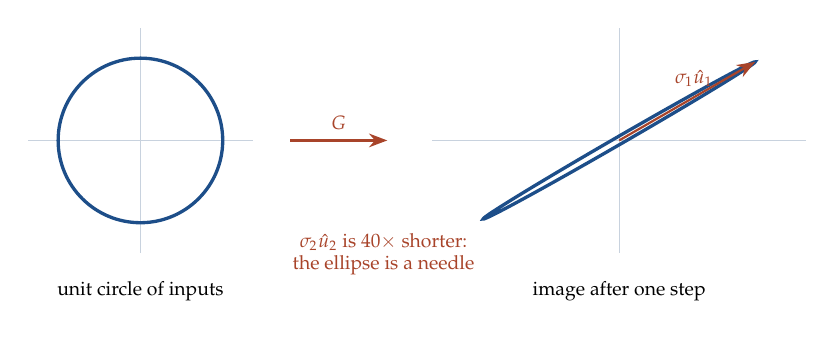
\begin{tikzpicture}[>=Stealth, scale=0.95]
  % unit circle
  \begin{scope}[shift={(0,0)}]
    \draw[rule] (-1.5,0) -- (1.5,0);
    \draw[rule] (0,-1.5) -- (0,1.5);
    \draw[accent, very thick] (0,0) circle (1.1);
    \node[font=\scriptsize, below] at (0,-1.75) {unit circle of inputs};
  \end{scope}
  \draw[->, thick, warm] (2.0,0) -- (3.3,0) node[midway, above, font=\scriptsize, warm] {$G$};
  % ellipse
  \begin{scope}[shift={(6.4,0)}]
    \draw[rule] (-2.5,0) -- (2.5,0);
    \draw[rule] (0,-1.5) -- (0,1.5);
    \draw[accent, very thick, rotate=30] (0,0) ellipse [x radius=2.1, y radius=0.051];
    \draw[->, warm, thick, rotate=30] (0,0) -- (2.1,0)
      node[pos=0.55, above, font=\scriptsize, warm, sloped] {$\sigma_1 \hat{u}_1$};
    \node[font=\scriptsize, below] at (0,-1.75) {image after one step};
  \end{scope}
  \node[font=\scriptsize, warm, align=center] at (3.25,-1.52)
    {$\sigma_2 \hat{u}_2$ is $40\times$ shorter:\\ the ellipse is a needle};
\end{tikzpicture}
\end{center}

\noindent
A single $\eta$ has to be small enough to keep $\sigma_{1}$ under control, which means
almost nothing happens along $\hat{v}_{2}$. This is the condition-number problem of
Section A1 again, but now inside a single weight matrix. A per-coordinate method such as
Adam cannot detect it, because it sees $D$ separate numbers rather than the matrix they
form.

\begin{keybox}
\textbf{The idea behind Muon.} If the update acts with very different strength in
different directions, we can flatten its spectrum before applying it so that every
direction receives a comparable step. We stopped at this point in the lecture. How the
flattening is done in practice, and whether it holds up at scale, is covered in this
week's reading (Jordan et al.; Liu et al.).
\end{keybox}

% ================================================================ closing
\section*{Where this leaves us}
\addcontentsline{toc}{section}{Where this leaves us}

The universal approximation theorem tells us a good network exists, and leaves two
questions open. We spent today on the first. One idea runs through A1--A7: a single
learning rate $\eta$ is being asked to do a job that varies by direction, whether across
parameters (A4--A6), across time (A2, A5) or within a single weight matrix (A7). Much of
the progress in optimisation comes from finding another place where that assumption
fails.

\medskip
\noindent
Next lecture we look at the gradient itself, $\nabla_\theta \Loss$, and then at
generalisation: dropout, weight decay, grokking and double descent, and what they tell us
about optimisation.

\vspace{0.6em}
\noindent\textbf{\color{accent}This week's reading.}
Jordan et al., \emph{Muon} \textbullet\ Liu et al., \emph{Muon is scalable}
(arXiv:2502.16982).

\end{document}
